\documentclass[a4paper,12pt]{article}
\usepackage[english,ukrainian,russian]{babel}
\linespread{1}
\usepackage{ucs}
\usepackage[utf8]{inputenc}
\usepackage[T2A]{fontenc}
\usepackage[paper=portrait,pagesize]{typearea}
\usepackage{amsmath}
\usepackage{bigints}
\usepackage{amsfonts}
\usepackage{graphicx}
\usepackage{amssymb}
\usepackage{cancel}
\usepackage{gensymb}
\usepackage{multirow}
\usepackage{rotate} 
\usepackage{pdflscape}
\usepackage{bigstrut}
\usepackage[pageanchor]{hyperref}
\usepackage{chngpage}
\usepackage{fancybox,fancyhdr}
\newcommand\tab[1][1cm]{\hspace*{#1}}
\newcommand{\RomanNumeralCaps}[1]{\MakeUppercase{\romannumeral #1}}
\usepackage[left=20mm, top=20mm, right=15mm, bottom=15mm, nofoot]{geometry}

\usepackage{verbatim}
\usepackage{enumerate}
\usepackage{listings}
\usepackage{xcolor}

\definecolor{codegreen}{rgb}{0,0.6,0}
\definecolor{codegray}{rgb}{0.5,0.5,0.5}
\definecolor{codepurple}{rgb}{0.58,0,0.82}
\definecolor{backcolour}{rgb}{0.95,0.95,0.92}

\lstdefinestyle{mystyle}{
	backgroundcolor=\color{backcolour},   
	commentstyle=\color{codegreen},
	keywordstyle=\color{blue},
	numberstyle=\tiny\color{codegray},
	stringstyle=\color{red},
	basicstyle=\ttfamily\footnotesize,
	breakatwhitespace=false,         
	breaklines=true,                 
	captionpos=b,                    
	keepspaces=true,                 
	numbers=none,                    
	numbersep=5pt,                  
	showspaces=false,                
	showstringspaces=false,
	showtabs=false,                  
	tabsize=4,
	frame=shadowbox
}

\lstset{style=mystyle}

% Language "Assembler"
\lstdefinelanguage{assembler}{
    keywords={MOV, LDR, CMP, BEQ, BLT, SUB, B, ADD, STR. DCD, LSL},
    sensitive=true,
    comment=[l]{;},  % Коментарі починаються з ;
    morestring=[b]",  % Рядки в лапках
    morestring=[b]',  % Рядки в одинарних лапках
}
\lstset{
    language=assembler,          % Встановлюємо мову
    basicstyle=\ttfamily,        % Шрифт для коду
    keywordstyle=\color{blue},   % Стиль для ключових слів
    commentstyle=\color{green},  % Стиль для коментарів
    stringstyle=\color{red},     % Стиль для рядків
    numbers=left,                % Номери рядків зліва
    numberstyle=\tiny,           % Стиль номерів рядків
    stepnumber=0,                % Номери для кожного рядка
    numbersep=5pt,               % Відстань до номера рядка
    frame=single,                % Рамка навколо коду
}

\begin{document}
    \pagestyle{fancy}
    \fancyhead{}
    \fancyhead[R]{ФІ-12 Завалій Олександр}
    \begin{center}
        \large{\textbf{Міністерство освіти і науки України\\
                Національний технічний університет України\\
                «Київський політехнічний інститут імені Ігоря Сікорського»\\
                Навчально-науковий Фізико-технічний інститут}}\\
        \hfill \break \hfill \break \hfill\break \hfill \break \hfill \break \hfill \break \hfill \break
        \hfill \break \hfill \break \hfill \break
        \begin{center}
            \normalsize{\textbf{Архітектура комп'ютерних систем\\
            Комп’ютерний практикум\\
            Робота №3}}
        \end{center}
    \end{center}
    \hfill \break \hfill \break \hfill \break \hfill \break \hfill \break \hfill \break \hfill \break
    \hfill \break \hfill \break \hfill \break \hfill \break 
    \begin{flushright}
        \large{ \hspace{35pt} Виконав:\\
            студент групи ФI-12\\
            Завалій Олександр\\} 
        \large{ \hspace{35pt} Перевірив:\\
        Козленко О.В.} 
    \end{flushright}
    \hfill \break \hfill \break \hfill \break \hfill \break \hfill \break \hfill \break \hfill \break
    \hfill \break
    \begin{center} \textbf{Київ-2024} \end{center}
    \thispagestyle{empty}

\newpage
    \begin{center}
        \section*{\bfseries{Робота №3.\\
        Основи побудови програми на асемблері в архітектурі ARM
    }}
    \end{center}
    \textbf{Мета:} \\
    \hangindent=1.5cm 
    \hangafter=+1 \noindent
    Ознайомитися з створенням базової програми на мові асемблер для архітектури ARM \\
    \begin{center}
        \Large{Варіант №4}
    \end{center}
    Зміст індивідуального завдання:
    \begin{enumerate}
        \item Завантажити \href{https://github.com/tomcl/V2releases}{VisUAL2}.
        \item Ознайомитись з теоретичними положеннями.
        \item Визначити змінні, занести відповідні значення у регістри та організувати цикл
        роботи для архітектури ARM згідно свого варіанту: \\
        Дано натуральні числа $n, a_1,\:...,\:a_n$. Отримати середнє арифметичне тих
        членів послідовності $a_1,\:...,\:a_n$ які при діленні на $5$ дають залишок $1$ чи $2$.
        \item Підготувати звіт і представити на захист.
    \end{enumerate}

\newpage
    \begin{center}
        \Large{Code}
    \end{center}
    \begin{lstlisting}[language=assembler]
ENTRY              
        LDR     R0, =ASize
        LDR     R1, [R0]
        LDR     R2, =Array
        MOV     R3, #0
        MOV     R4, #0
        MOV     R5, #0

compareLoop        
        CMP     R3, R1
        BEQ     endLoop

        LDR     R6, [R2, R3, LSL #2]
        MOV     R7, R6

calculateRemainder 
        CMP     R7, #5
        BLT     checkRemainder
        SUB     R7, R7, #5
        B       calculateRemainder

checkRemainder     
        CMP     R7, #1
        BEQ     addToSum
        CMP     R7, #2
        BEQ     addToSum

nextElement        
        ADD     R3, R3, #1
        B       compareLoop

addToSum           
        ADD     R4, R4, R6
        ADD     R5, R5, #1
        B       nextElement

endLoop            
        CMP     R5, #0
        BEQ     storeZero

        MOV     R0, R4
        MOV     R1, R5
        MOV     R2, #0
        MOV     R3, #0
    \end{lstlisting}

\newpage
    \begin{lstlisting}[language=assembler]
calculateAverage   
        CMP     R1, #0
        BEQ     storeAverage

divisionLoop       
        CMP     R0, R1
        BLT     storeAverage
        SUB     R0, R0, R1
        ADD     R2, R2, #1
        B       divisionLoop

storeAverage       
        LDR     R0, =Result
        STR     R2, [R0]
        B       stopExecution

storeZero          
        MOV     R2, #0
        LDR     R0, =Result
        STR     R2, [R0]
        B       stopExecution

stopExecution      
        B       stopExecution 

ASize              DCD     6
Array              DCD     3, 7, 12, 21, 26, 31
Result             DCD     0

    \end{lstlisting}
    \begin{figure}[h!]
        \begin{minipage}[h]{1\linewidth}
            \centering
            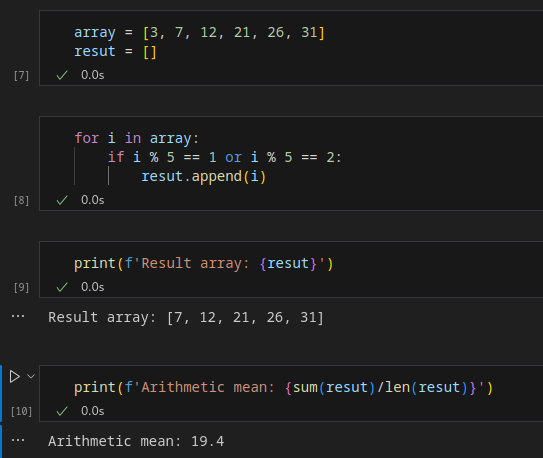
\includegraphics[width=0.6\linewidth]{Prt sc/python_code_1.png}  
        \end{minipage}
    \end{figure}

\newpage
    \begin{center}
        \Large{Results}
    \end{center}
    \begin{figure}[h!]
        \begin{minipage}[h]{1\linewidth}
            \centering
            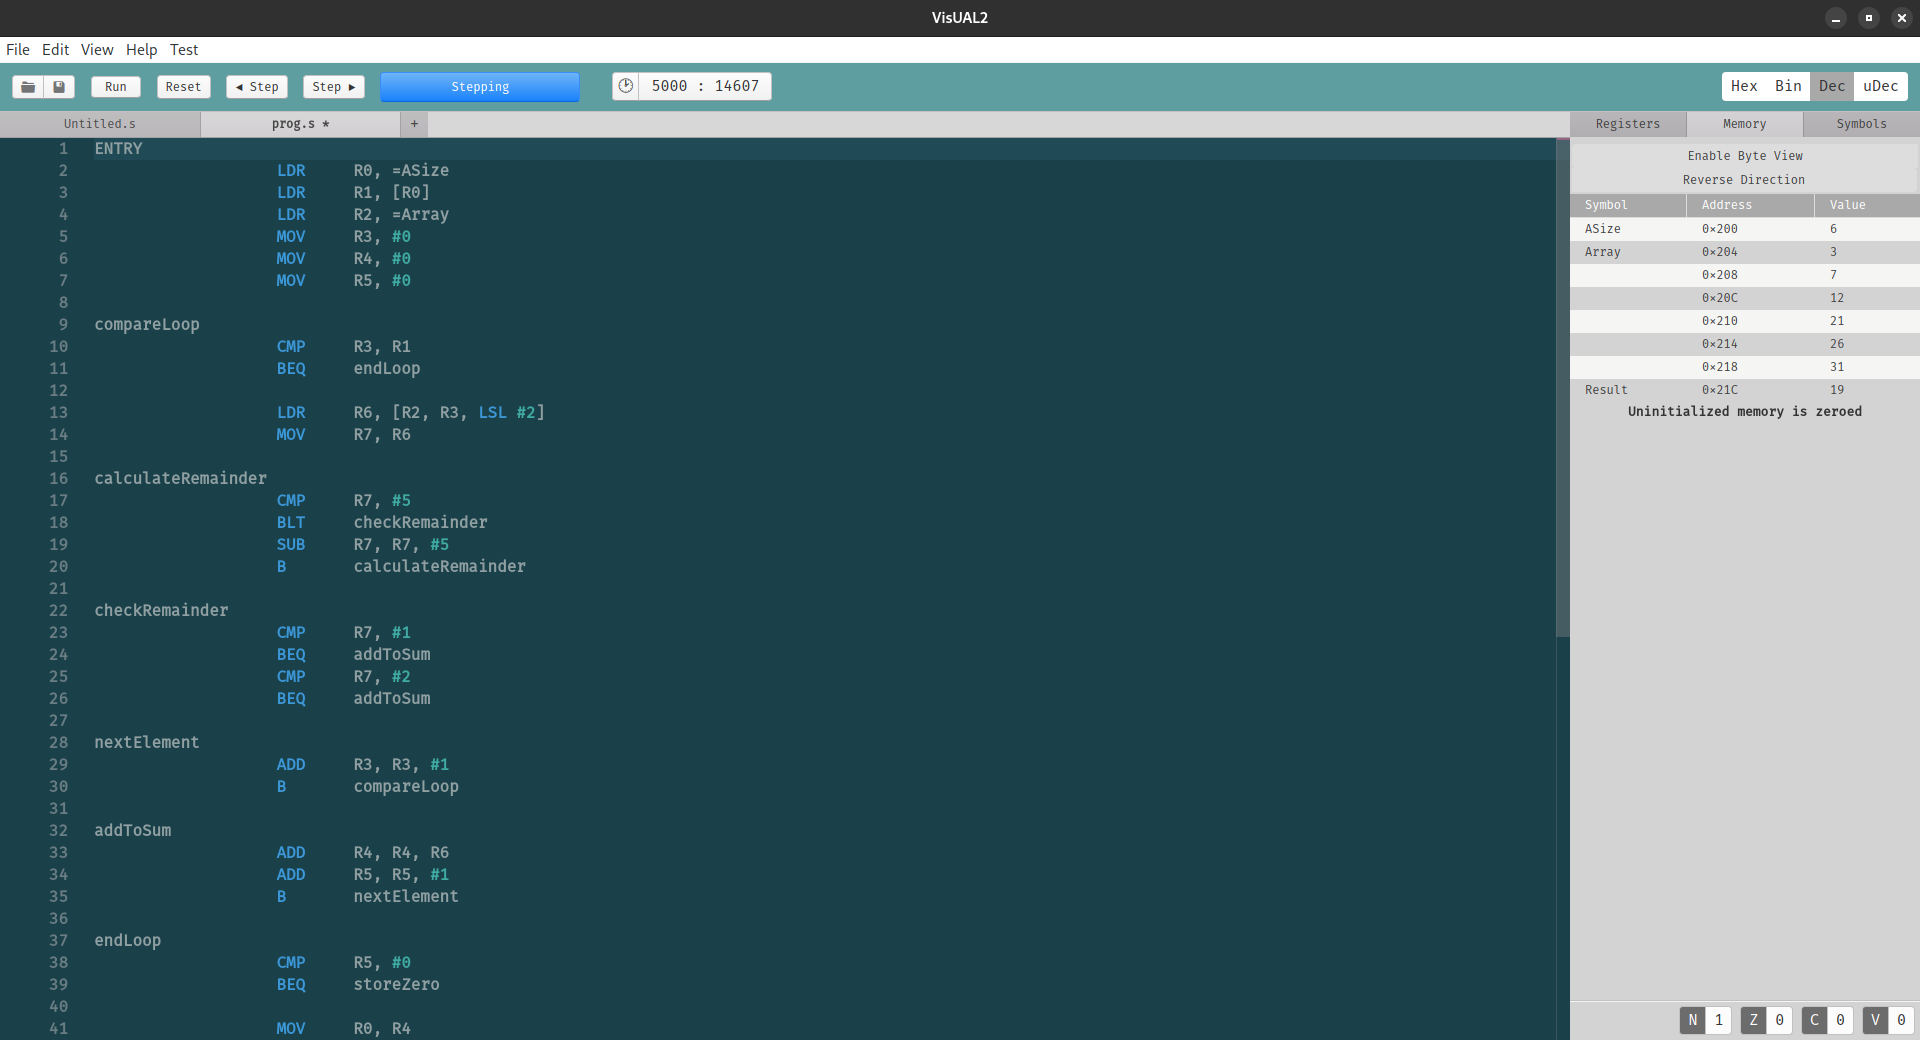
\includegraphics[width=1\linewidth]{Prt sc/1_1.png}  
        \end{minipage}
    \end{figure}
    \begin{figure}[h!]
        \begin{minipage}[h]{1\linewidth}
            \centering
            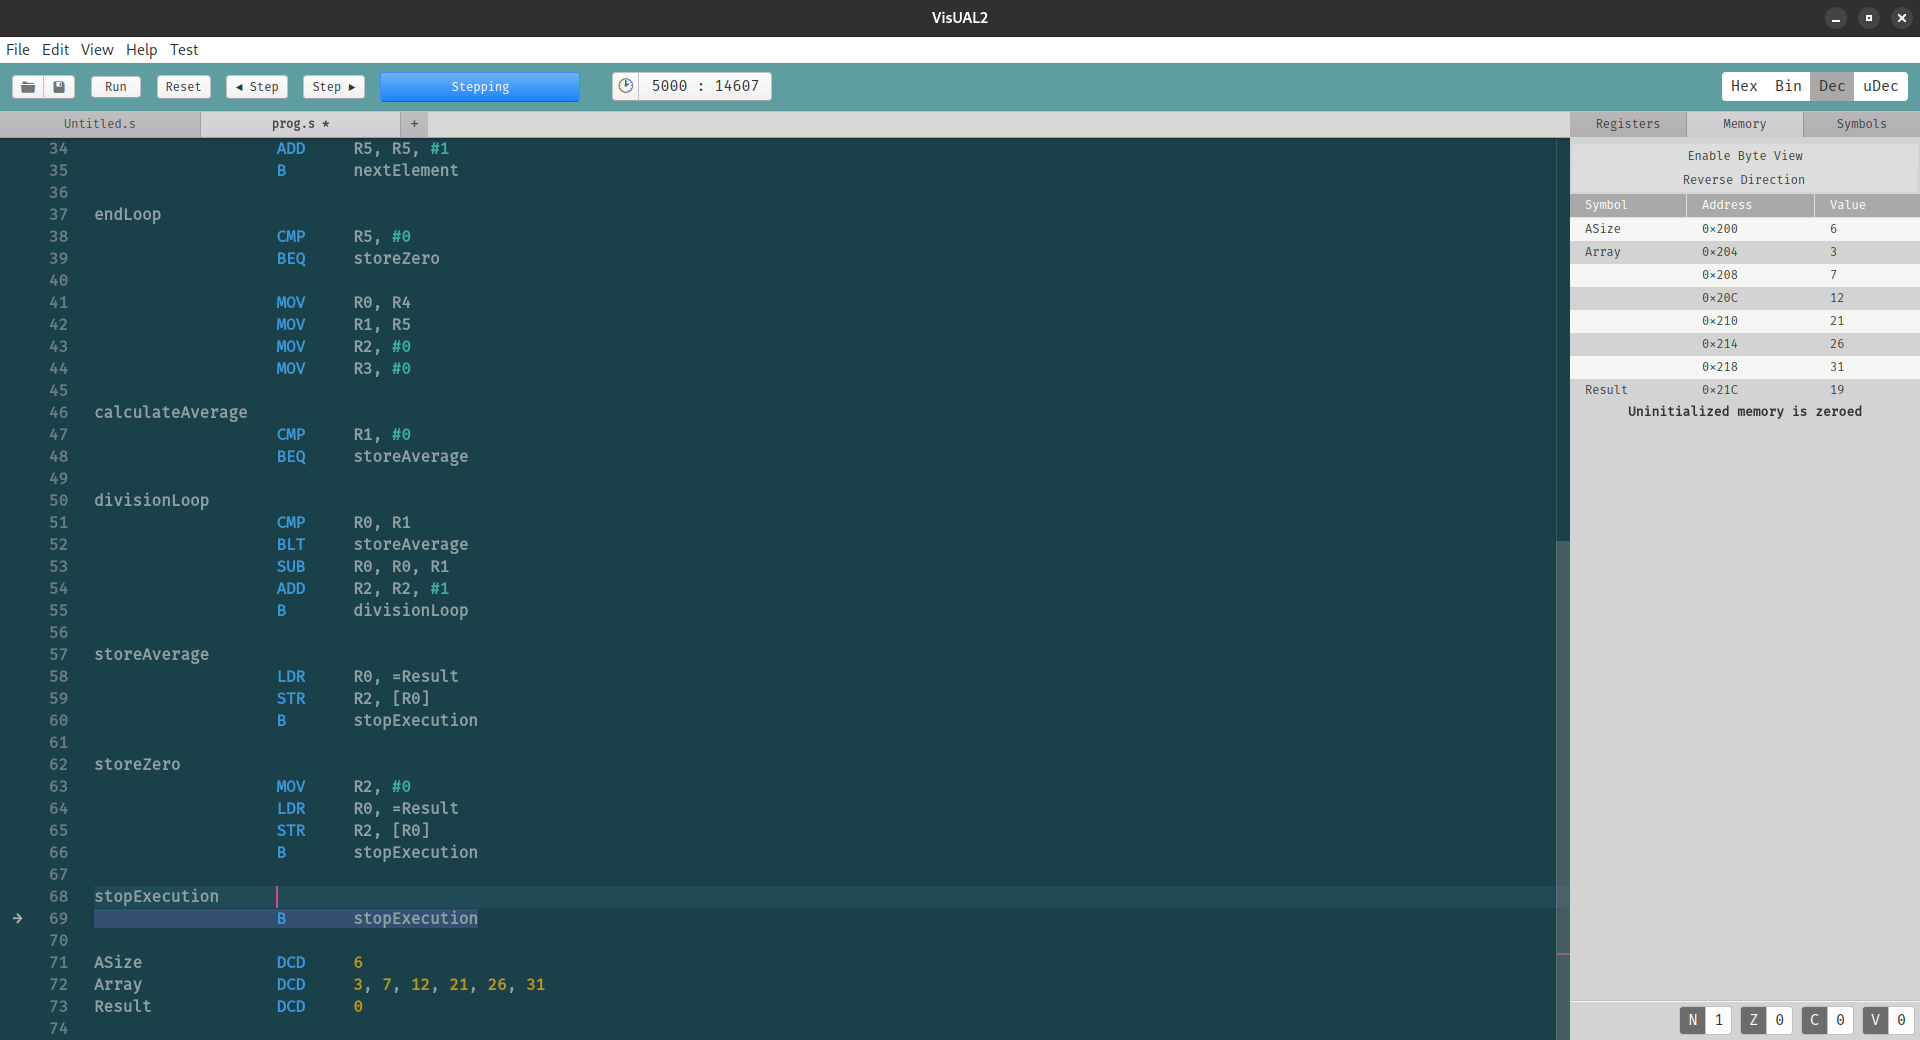
\includegraphics[width=1\linewidth]{Prt sc/1_2.png}  
        \end{minipage}
    \end{figure}
    Результати роботи програм співпадають.

\end{document}